\chapter[Introduction]{Introduction}
%\addcontentsline{toc}{chapter}{Chapter 1\\Introduction}
\label{chapter:introduction}
\pagenumbering{arabic}

In chapter \ref{chapter:introduction},  present spectrum scarcity problem as the background of this thesis and technology proposed for solution is described. Aslo, the overview of this thesis and purpose is described. 
\section{Background}
 Due to the rapid development of wireless communication systems, a demand on sprectrum resource for communication has increased explosively. Because the data rate and perfomance of the wireless communication system, such as mobile phone, are improved, it leads to a serious sprectrum scarcity problem.

 From Fig. \ref{fig:Cisco}, reference \cite{ref:Cisco} predicts that Global mobile data traffic will increase nearly tenfold between 2014 and 2019 and mobile data traffic will grow at a compound annual growth rate (CAGR) of 57 percent from 2014 to 2019, reaching 24.3 exabytes per month by 2019. 
\begin{figure}[!htp]
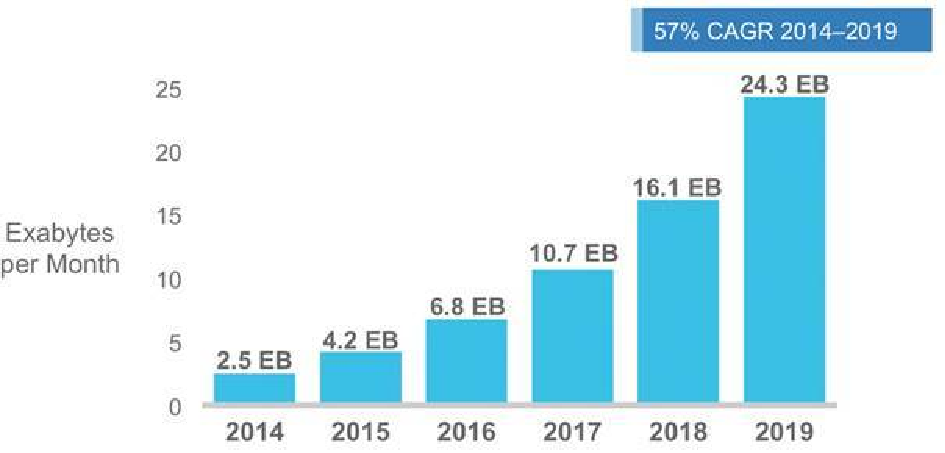
\includegraphics[width=150mm,clip]{traffic_trend.pdf}
\caption{Cisco Forecasts 24.3 Exabytes per Month of Mobile Data Traffic by 2019}
\label{fig:Cisco}
\end{figure}
In addition to the increasement of the data traffic, a fixed resource allocation method as the current spectrum allocation policy, which is utilized for avoiding harmful interference toward licensed systems with each other, is also considered as a major reason for the scarcity of the spectrum resource. As a reason, almost linear increasing demand on necessary bandwidth for communication leads to a difficult allocation for new systems. From Fig. \ref{fig:MIC} reported from Ministry of Internal Affairs and Communications(MIC) in Japan government\cite{ref:MIC}, it is shown that most of the spectrum resources has already been allocated. Thus, the lack of spectrum resources has become a serious problem.
\begin{figure}[!htp]
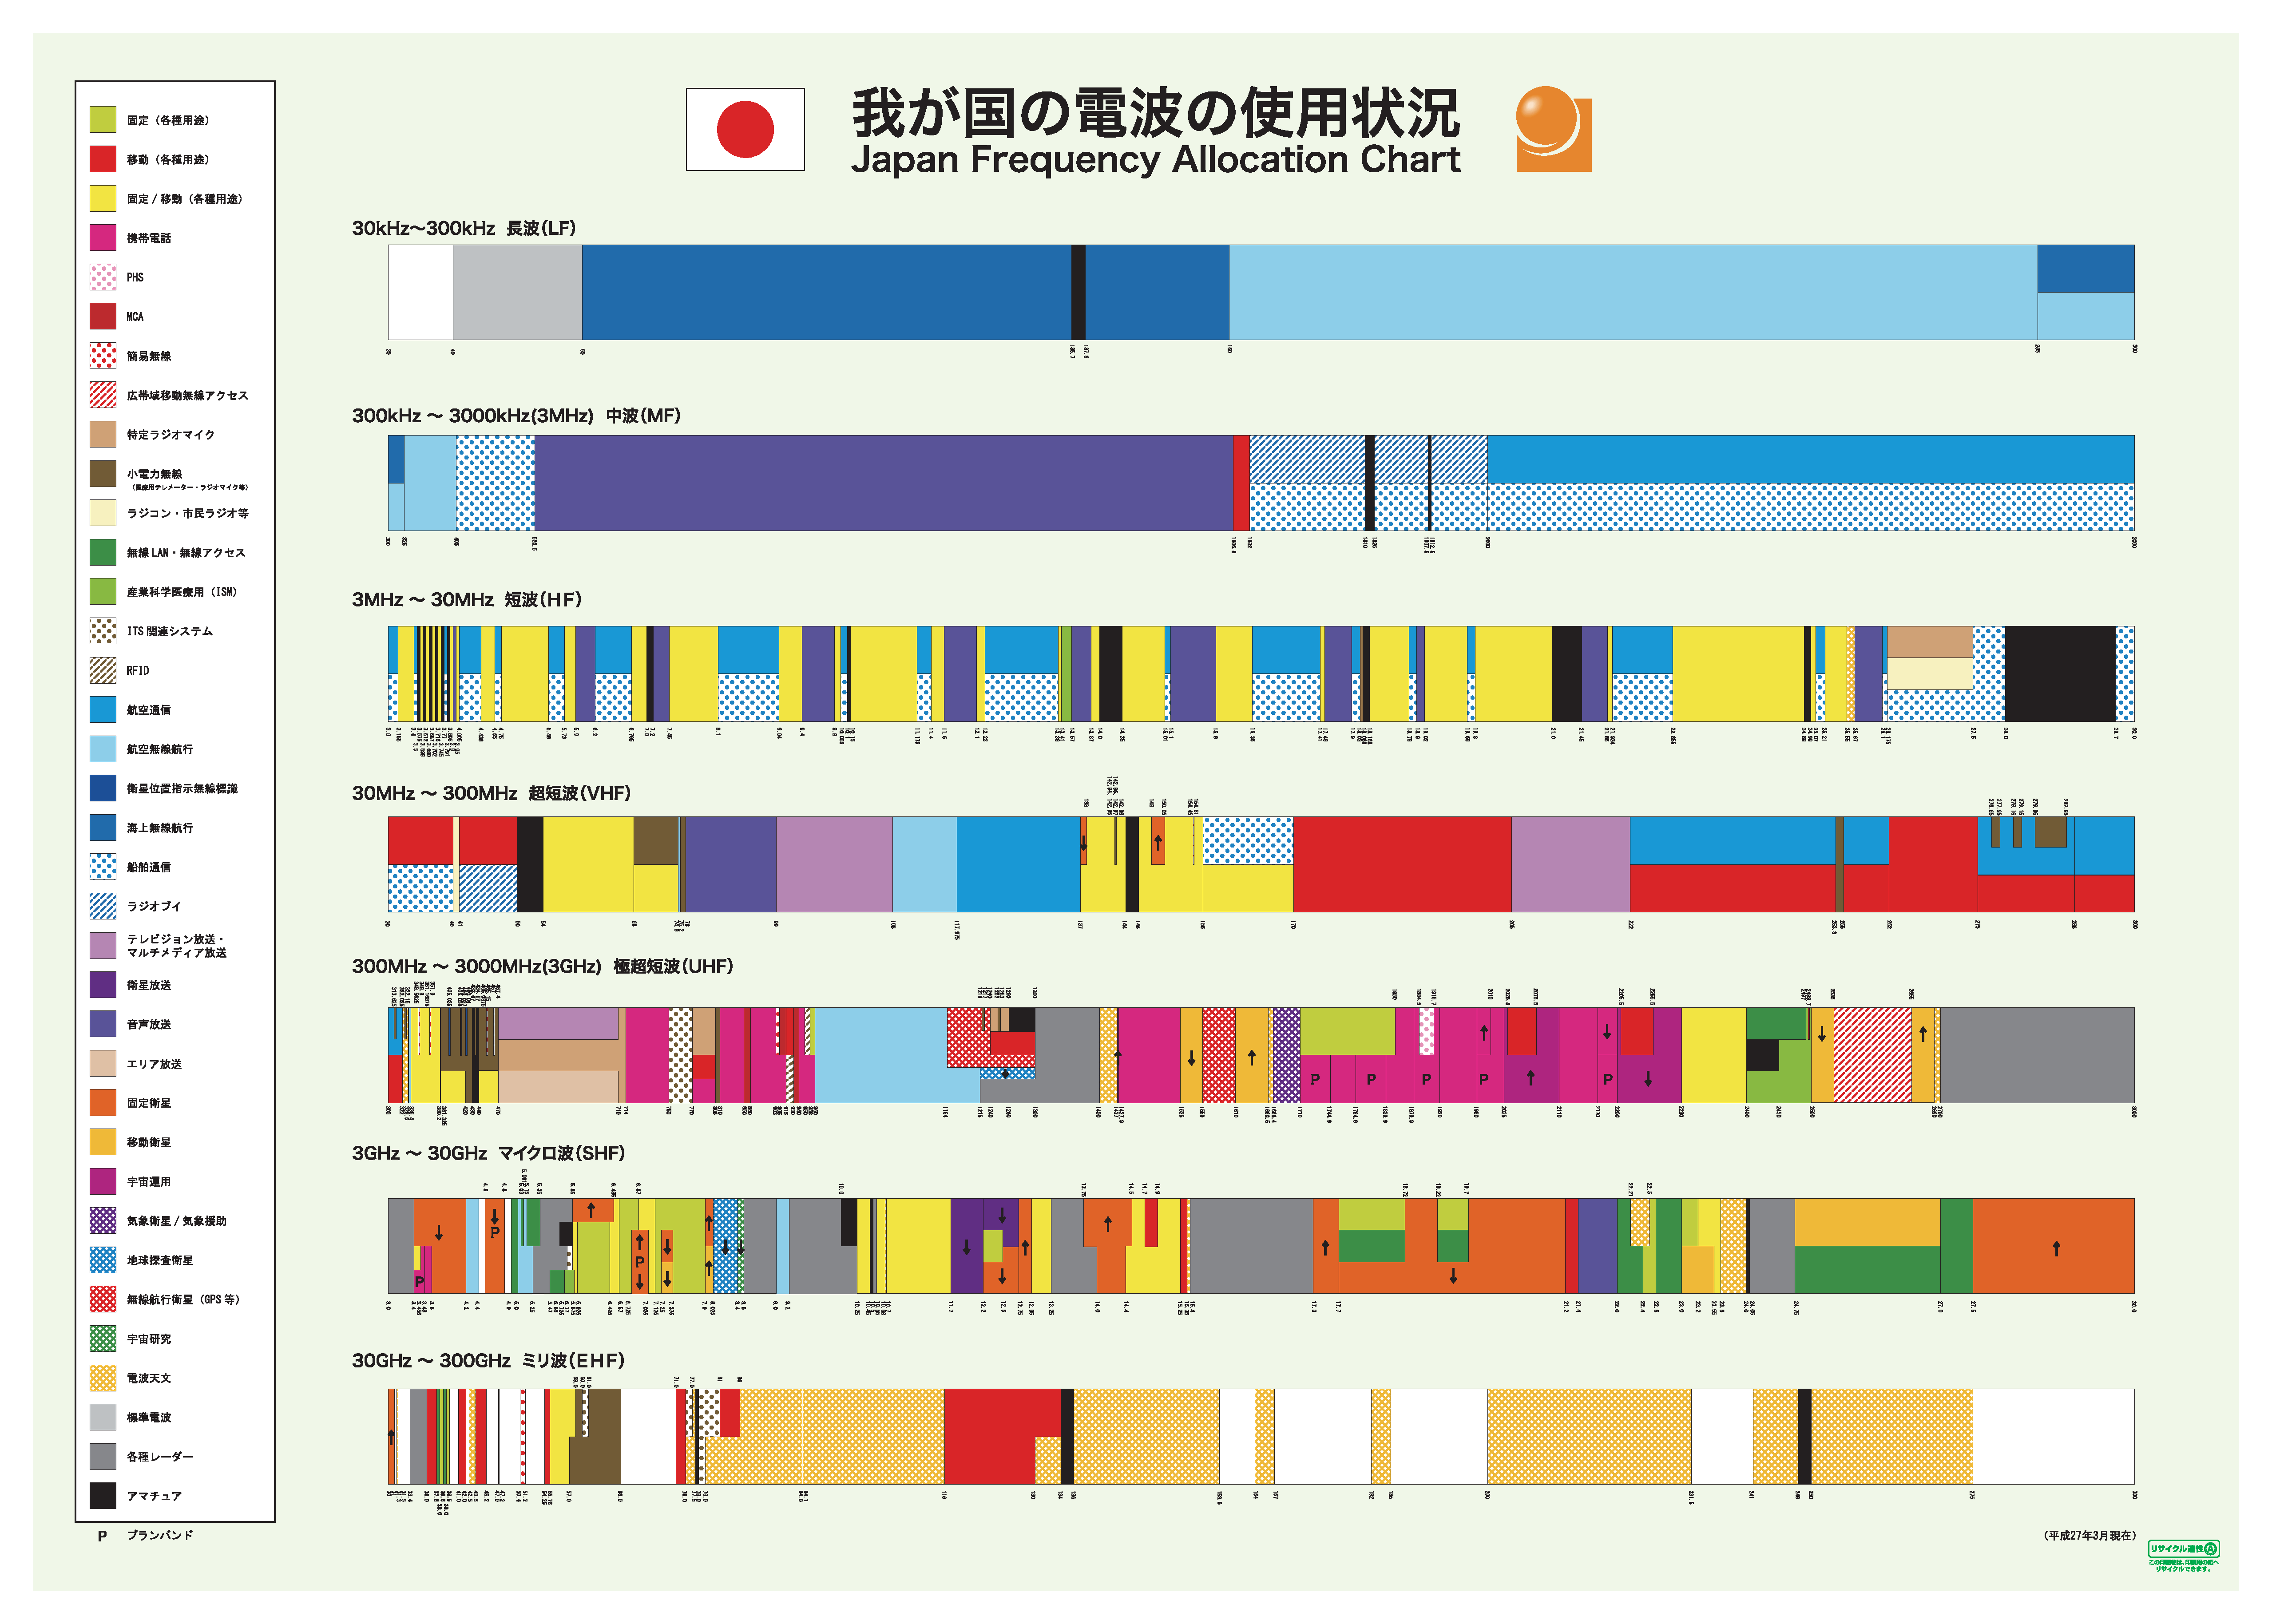
\includegraphics[width=150mm,clip]{frequency_alloc.pdf}
\caption{Japanese Frequency Allocation Chart.}
\label{fig:MIC}
\end{figure}

Since the finite spectrum resources are not able to fulfill the expoential growth of demand on traffic, it is necessary to review the present spectrum policy with fixed resource allocation for the next generation wireless communication sysytems and a effecient spectrum utilization turns to be a key problem. 

There are 2 main methods to ensure the bandwidth for new systems. Firstly, a spectrum arrangement on the whole wireless communication systems is utilized to extend available bandwidth. In 2011, an arrangement on television broadcasting is executed with switching to digital television broadcasing. However, it is not available for supporting the expoential growth of the data traffic and the number of systems. Second, an efficient and dynamic utilization method of bandwidth is considered to extend the probability for the future wireless communication systems, which is attracted attention as effective solution to the shortage of spectrum resources. 

According to the report \cite{ref:FCC} from Federal Communications Commission(FCC), actual spectrum usage on the licensed band is lack of balance in both temporal and spatial domain and instantaneous usage efficiency remains at 15\%~80\% even under crowd environment, such as urban areas, which means that an unused White Space(WS) exists even under temporal and spatial varying envrionment. However, it is not allowed to utilize White Space by other licensed or unlicensed systems based on current radio regulations.

\section{Spectrum Sharing Trend and Problem}
Cognitive Radio(CR)\cite{ref:Haykin} has been recognized as a promising solution to address the problem for improving the utilizetion of spectrum for various wireless applications. In a CR system from Fig.\ref{fig:CR_time} and \ref{fig:CR_space}, it allows the Secondary Users (SUs) to opportunistically utilize the temporal and/or spatial unused spectrum holes without causing interference to Primary Users (PUs). While SUs can occupy avaliable spectrum holes as long as the corresponding PU is inactive, they must immediately evacuate the band as soon as the corresponding PU appears.

\begin{figure}[!htp]
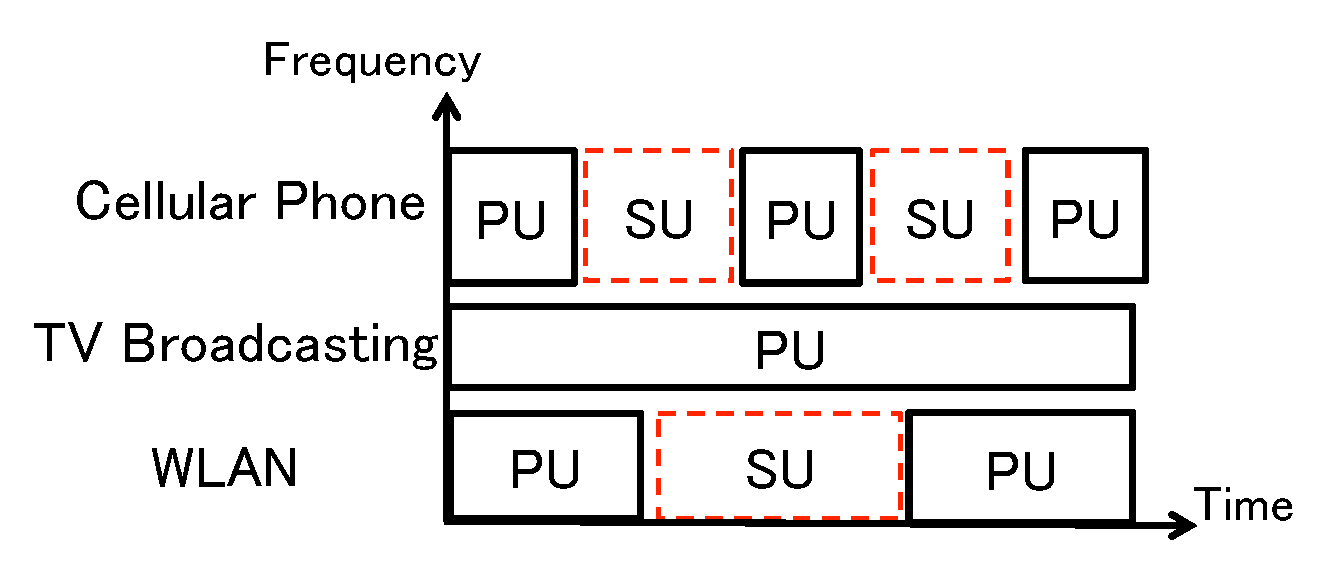
\includegraphics[width=150mm,clip]{CR_time.eps}
\caption{Coexsitance between PU and SU in time domain.}
\label{fig:CR_time}
\end{figure}

\begin{figure}[!htp]
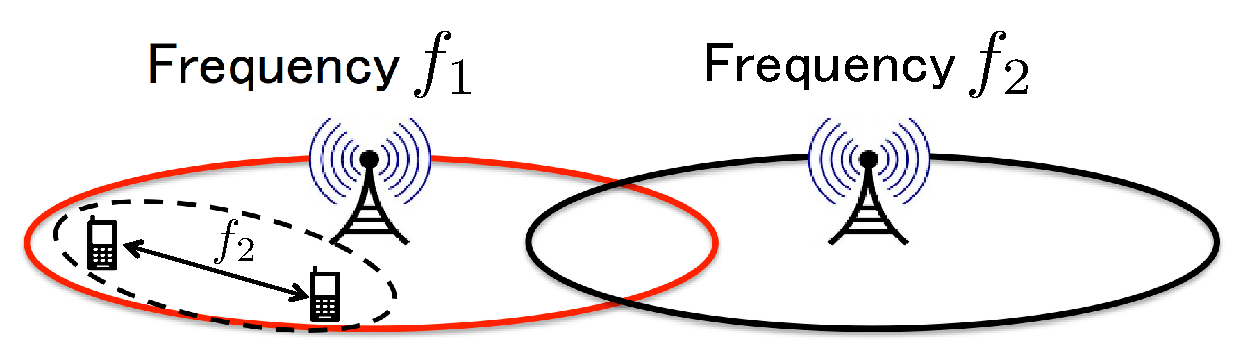
\includegraphics[width=150mm,clip]{CR_space.eps}
\caption{Coexsitance between PU and SU in space domain.}
\label{fig:CR_space}
\end{figure}

One of the main chanllenges is to intelligently determine ongoing PU activity to avoid interferece toward PU. SUs can evacuate the band without affecting PU’s activity and opportunistically access the spectrum to maximize the spectrum usage if the information about PU can be obtained in advance. Hence, more information about PU leads to more effective spectrum usage for SUs, and an external device for provding information of PU is necessary. One of the main chanllenges is to intelligently determine ongoing PU activity to avoid interferece toward PU. SUs can evacuate the band without affecting activity of PU and opportunistically access the spectrum to maximize the spectrum usage if the information about PU can be obtained in advance. Hence, more information about PU leads to more effective spectrum usage for SUs, and an external device for providing information of PU is necessary. However, it is difficult for SU to obtain the information about activity of PU individually according to the position of SU and it may leads a performation degradation on PU protection.

The idea of Spectrum Database has been studied for assisting SUs to effectively reuse the spectrum. SUs can access the database to obtain the surrounding radio environment information and optimize their own parameters,
such as modulation, transmitting power and so on. Federal Comminication Committee (FCC) has been considered a propagation model-based spectrum database to provide the spectrum available information whether the spectrum locating SU can be used or not [3]. The model-based database has to set a large margin to avoid interference to PU because the realistic radio environment with considering the effect of surrounding obstacles cannot be considered. Therefore, there is a limit to improve the spectrum utilization efficiency.

Authors in \cite{ref:fujii_Database} proposed a measurement-based spectrum database as a realistic method. The measurement-based database generates the database information by gathering the measuring received power at SUs, which are inactive for communication. Then the real radio propagation situation can be known and more accurate information at SU location can be provided. Then, SUs access to the database with their own location information and download the responding average received signal power at the SU location as shown in Fig.\ref{fig:Database}.
\begin{figure}[!htp]
\begin{center}
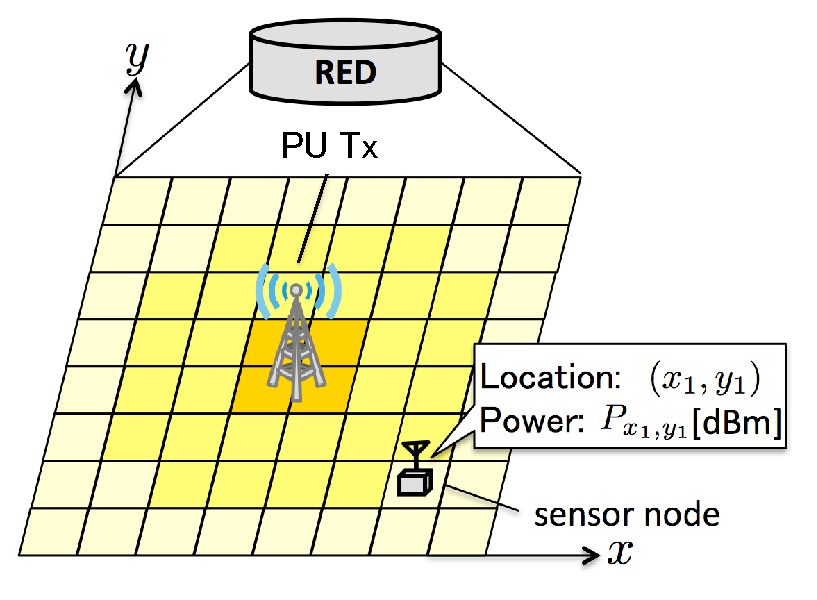
\includegraphics[width=125mm,clip]{database.eps}
\caption{Measurement-based Spectrum Database.}
\label{fig:Database}
\end{center}
\end{figure}

The database is constructed by using reported measurement results of averaged sampling value in each sensor node like energy detection spectrum sensing algorithm to calculate the average received signal power at each location. However, it is only appropriate under the assumption that the PU status is always ON. For example, in \cite{ref:ON1}\cite{ref:ON2}, the channel scenario is not considering primary user traffic during the sensing period. If there is a state transition from ON to OFF, sensor node will report the wrong received signal power to the database, which leads to low reliability and performance. Thus, it is necessary to detect PU’s state transition and extract the ON part only to the database to improve the reliability of database. In \cite{ref:quickest}, single status change of primary user is focused.

\section{Purpose}
In this thesis, we focus on a distribution transition between the ON status and OFF status, CUSUM (cumulative sum) algorithm \cite{ref:CUSUM} and GLR (Generalized Likelihood Ratio) algorithm \cite{ref:GLR} are used to detect the rise up point and rise down point, which is status change point from OFF to ON and ON to OFF. Finally, only ON power can be extracted with using the detected transition point and the sensing error reduction is possible. 

The remainder of this thesis is organized as follows. The overview of Cognitive Radio and Spctrum Sharing with Spectrum Database is introduced in Chapter \ref{chapter:CR}. In Chapter \ref{chapter:Database} the basic sensing method for calculating the reported information is presented as a measurement-based spcetrum database construction metrics and the problem of Spectrum database construction is described in detail. Chapter \ref{chapter:Propose} proposes the active period detection method of primary signal for spectrum database in detail and the simulation results and performance evaluation are discussed in Chapter \ref{chapter:Result}. Finally, Chapter \ref{chapter:Conclusion} concludes the thesis.
